\documentclass[aspectratio=169]{beamer}
\RequirePackage{indentfirst,polski}
\usepackage[utf8]{inputenc}

\setbeamerfont{normal text}{size=\small}

\AtBeginDocument{\usebeamerfont{normal text}}

\geometry{paperwidth=140mm}

\input ../thesis/macros.sty

%%%%% WLASNE DODATKOWE PAKIETY
\usepackage{amsmath}
\usepackage{amssymb}
\usepackage{stmaryrd} % For \llbracket
\usepackage{mathpartir}
\usepackage{mathtools}
\usepackage{listings}
\usepackage{semantic}
\usepackage{sourcecodepro}
% \usepackage{enumitem}
\usepackage{tabularx}
\usepackage{makecell}
\usepackage{mdframed}
\usepackage{hyperref}
\usepackage{subcaption}
\usepackage[toc,page]{appendix}
\usepackage{multicol}
\usepackage{multirow}
\usepackage{graphicx}
\usepackage{pgf}
\usepackage{tikz-qtree}
\usepackage{graphicx}
\graphicspath{ {./images/} }

%%%%% WŁASNE DEFINICJE I POLECENIA
\definecolor{codegreen}{rgb}{0,0.6,0}
\definecolor{codegray}{rgb}{0.5,0.5,0.5}
\definecolor{codepurple}{rgb}{0.58,0,0.82}
\definecolor{backcolour}{rgb}{0.95,0.95,0.92}
\lstdefinestyle{ocamlstyle}{
    commentstyle=\color{codegreen},
    escapebegin=\color{black},
    keywordstyle=\color{magenta},
    numberstyle=\tiny\color{codegray},
    stringstyle=\color{codepurple},
    basicstyle=\ttfamily\footnotesize,
    breakatwhitespace=false,
    breaklines=true,
    captionpos=b,
    keepspaces=true,
    numbersep=5pt,
    showspaces=false,
    showstringspaces=false,
    showtabs=false,
    tabsize=2
}
\lstset{style=ocamlstyle, basicstyle=\ttfamily\footnotesize}
\lstdefinelanguage{OCaml}[]{caml}{
    morekeywords={val, ProofEnv, otherwise, private},
    otherkeywords = {|>, \%>, +=, -=, ->, ::}
}
\renewcommand{\sc}[1]{\textsc{\small{#1}}}
\renewcommand{\tt}[1]{\texttt{\small{#1}}}
\newcommand{\lstt}[1]{\text{{\lstinline[columns=fixed,mathescape]|#1|}}}
\renewcommand{\it}[1]{\textit{#1}}
\newcommand{\aequiv}{\ensuremath{=_\alpha}}
\newcommand{\solverRule}{\vdash}
\newcommand{\NeqAtoms}{\tt{neq\_atoms}}
\newcommand{\Fresh}{\tt{fresh}}
\newcommand{\VarShape}{\tt{var\_shape}}
\newcommand{\Shape}{\tt{shape}}
\newcommand{\Subshape}{\tt{subshape}}
\newcommand{\Symbols}{\tt{symbols}}
\newcommand{\TransferShape}{\tt{transfer\_shape}}
\newcommand{\Assumptions}{\tt{assumptions}}
\newcommand{\occurs}[2]{\ensuremath{ {#1}\text{ occurs in }{#2}}}
\newcommand{\stxoccurs}[2]{\ensuremath{ {#1}\text{ occurs syntactically in }{#2}}}
\newcommand{\pluseq}{\mathrel{+}=}
\newcommand{\minuseq}{\mathrel{-}=}
\newcommand{\shrep}[2][\icEnv]{\ensuremath{ #2_{#1}}}
\newcommand{\shenv}[2][\icEnv]{\ensuremath{ |#2|_{#1}}}
\newcommand{\fix}[3]{\ensuremath{\text{fix }#1(#2)\ofkind#3=}}\newcommand{\myatop}[2]{\ensuremath{\genfrac{}{}{0pt}{}{#1\hfill}{#2\hfill}}}
\newcommand{\scbrk}[2]{\myatop{\textsc{#1}}{\textsc{#2}}}
\newcommand{\hole}{\ensuremath{\bullet}}
\newcommand{\mdash}{\,---\,}
\def\-{{\mdash}}
\newcommand\fForallProp[2]{\forall_{#2} #1 .}
\newcommand\fExistsProp[2]{\exists_{#2} #1 .}
\newcommand{\rel}[2][\Gamma;C]{\ensuremath{#1\vdash#2}}
\newcommand{\types}[3][\Gamma]{\rel[#1]{#2 : #3}}
\newcommand{\interp}[2][\tmEnv]{\left\llbracket {#2} \right\rrbracket_{#1}}
\newcommand{\arr}{\rightarrow }
% \newcommand{\inference}[2]{\inference{ #1}{#2}}
\newcommand{\all}[1][x]{\ensuremath{\forall #1.\:}}
\newcommand{\exi}[1][x]{\ensuremath{\exists #1.\:}}
\newcommand{\karr}{\Rightarrow }
\newcommand{\lam}[1][x]{\lambda{#1}.\;}
\newcommand{\jgmnt[2]}[\cEnv;\Theta]{\ensuremath{#1 \vdash #2}}
\newcommand{\cjgmnt[2]}[\cEnv]{\ensuremath{#1 \vDash #2}}
\newcommand{\fv[1]}[\cEnv;\Theta]{\ensuremath{\operatorname{FV}(#1)}}

\newcommand{\inframe}[1]{\begin{tabular}{|c|} \hline \\[-3mm] {#1} \\[-3mm] \\ \hline \end{tabular}}
\newcommand{\fromany}[1]{
\begin{tikzpicture}[
  level distance=.75in,
  sibling distance=.15in,
  % auto,
  scale=0.85,
  edge from parent/.style={draw, thick,-latex},
  every tree node/.style={draw, align=center},
  grow'=down
]
\Tree
[.{\dots}
  \edge node[] { };
  [.{\ensuremath{#1}}
  ]
]
\end{tikzpicture}
}

\newcolumntype{L}{X}
\newcolumntype{C}{>{\centering\arraybackslash}X}
\newcolumntype{R}{>{\raggedleft\arraybackslash}X}

\usetheme{Copenhagen}
\usepackage{lmodern}
\usepackage[T1]{fontenc}
\usefonttheme{professionalfonts}

\title[Logika dla termów z wiązaniem zmiennych] %optional
{Logika dziedzinowa do wnioskowania \\ o~termach~z~wiązaniem zmiennych}

\subtitle{Domain-specific logic \\ for terms with variable binding}

\author
{Dominik Gulczyński \\ Promotor: dr Piotr Polesiuk}

\institute[UWr]
{
Uniwersytet Wrocławski \\
Wydział Matematyki i Informatyki \\
Instytut Informatyki
}

\date[2 Lutego 2024]
{Seminarium Zakładu Języków Programowania, 2 Lutego 2024}

\titlegraphic{\hfill
\includegraphics[width=1cm]{uwr-logo}}

\setbeamersize{
  text margin left=5mm,
  text margin right=5mm
}

\setbeamertemplate{footline}
{
  \hbox{\begin{beamercolorbox}[wd=1\paperwidth,ht=2.25ex,dp=1ex,right]{framenumber}%
      \usebeamerfont{framenumber}\insertframenumber{} / \inserttotalframenumber\hspace*{2ex}
    \end{beamercolorbox}}%
  \vskip0pt%
}
\setbeamertemplate{navigation symbols}{}

\begin{document}

\frame{\titlepage}

\begin{frame}
\frametitle{Dwa style prowadzenia rozumowań}
\begin{tabularx}{\textwidth}{LL}
  \begin{enumerate}
    \onslide<1->{\item Piszemy dla czytelnika}
    \onslide<2->{\item Pomijamy detale}
    \onslide<3->{\item Korzystamy z niejawnych założeń lub niedowiedzonych twierdzeń}
    \onslide<4->{\item Prowadzimy rozumowanie w konwencji nazw zmiennych Barendregta}
  \end{enumerate}
  &
  \begin{enumerate}
    \onslide<1->{\item Piszemy dla komputera}
    \onslide<2->{\item Musimy obsłużyć wszystkie detale}
    \onslide<3->{\item Korzystamy tylko z jawnych założeń lub i dowiedzonych twierdzeń}
    \onslide<4->{\item ?}
  \end{enumerate}
\end{tabularx}
\end{frame}

\begin{frame}
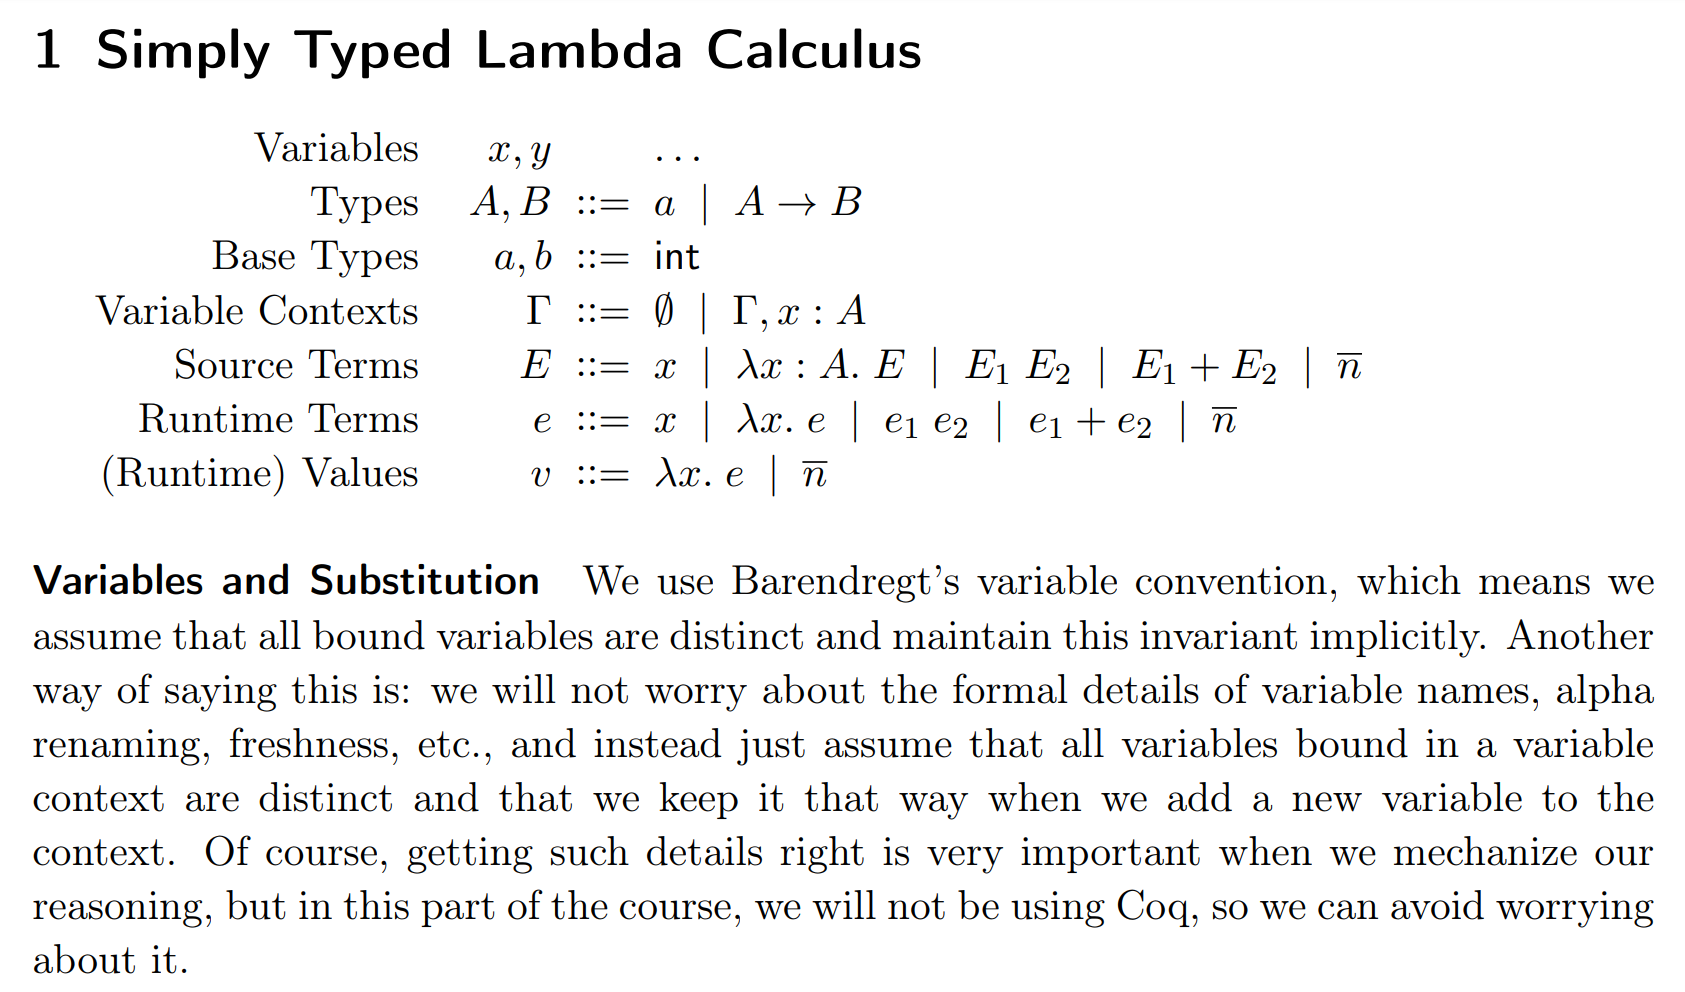
\includegraphics[width=\textwidth]{semantics}
{\footnotesize źródło: Semantics lecture notes 2019/2020, Derek Dreyer, Universität des Saarlandes}
\end{frame}

\begin{frame}
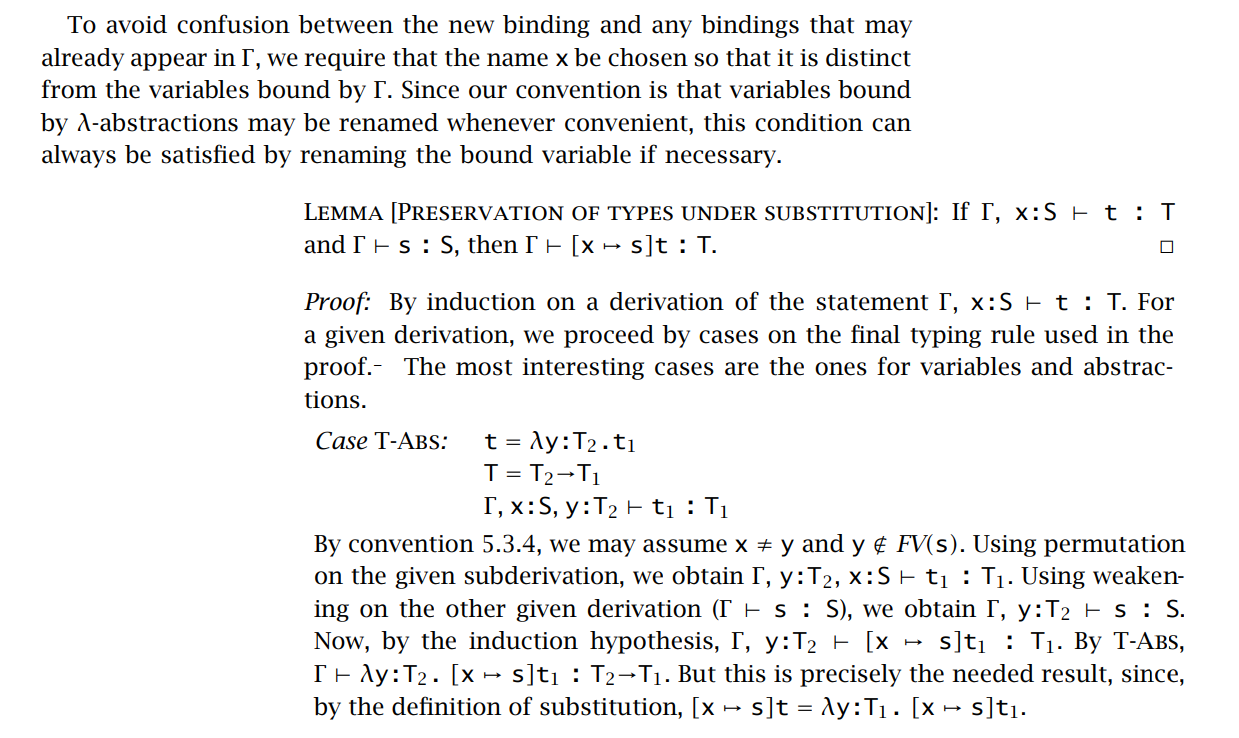
\includegraphics[width=\textwidth]{pierce-binding}
{\footnotesize źródło: Types and Programming Languages, Benjamin C. Pierce, MIT Press.}
\end{frame}

\begin{frame}
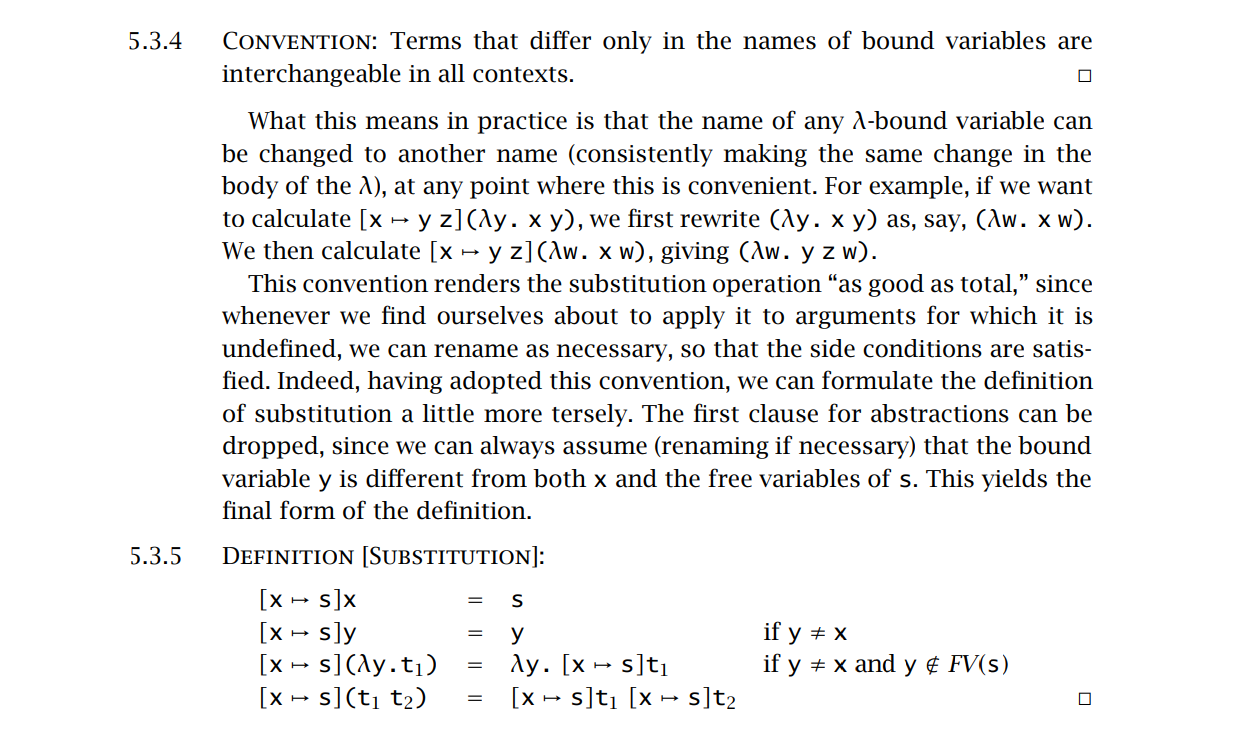
\includegraphics[width=\textwidth]{pierce-convention}
{\footnotesize źródło: Types and Programming Languages, Benjamin C. Pierce, MIT Press.}
\end{frame}

\begin{frame}
\frametitle{Rozwiązania problemu wiązania zmiennych w systemach formalnych}
% \begin{tabularx}{\textwidth}{LL}
  \begin{itemize}
  \onslide<1->{\item Rachunek kombinatorów}
  \onslide<2->{\item Reprezentacja De Bruijna}
  \onslide<3->{\item Higher-Order Abstract Syntax}
  \onslide<4->{\item Techniki nominalne}
  \end{itemize}
  % &
  % {\huge $\lambda x . e$}
% \end{tabularx}
\end{frame}

\begin{frame}
\frametitle{Logika nominalna}
  \begin{itemize}
  \item Rozszerzenie logiki pierwszego rzędu o narzędzia do formalizacji \\
i rozumowania na temat struktur syntaktycznych z wiązaniem nazw \\
  \item Matematyzacja pojęcia
``wystarczająco świeżych nazw'' zmiennych \\
  \item
  Opiera się o zamianę nazw i relację świeżości nazwy w termie.\\
  \end{itemize}
\begin{mdframed}[frametitle={\textnormal{\scriptsize \textbf{Andrew M. Pitts}, \textit{``Nominal logic, a first order theory of names and binding''}}:}]
{\footnotesize
Names of what? Names of entities that may be subject to binding by some of
the syntactical constructions under consideration. In Nominal Logic these sorts of
names, the ones that may be bound and hence that may be subjected to swapping
without changing the validity of predicates involving them, will be called atoms.
}
\end{mdframed}
\end{frame}

\begin{frame}
  \begin{tabularx}{\textwidth}{C}
    \hspace{9cm}
      $ t \; \deff \; a \mid \lambda a . t \mid t\;t$
    \\ \\
    \begin{tabular}{rcl}
    $\qquad\permswap{a}{b}{c}$ & $:=$
      & $ \begin{cases}
        a & \text{if } c = b \\
        b & \text{if } c = a \\
        c & \text{wpp.}
      \end{cases}$
      $\quad$
      \\
    \end{tabular}
    \begin{tabular}{rcl}
      $\qquad$
      $\permswap{a}{b}{(\lambda c . t)} $ & $:=$
      & $ \lambda (\permswap{a}{b}{c}) . (\permswap{a}{b}{t})$ \\
      $\permswap{a}{b}{(t_1\; t_2)} $ & $:=$
      & $ (\permswap{a}{b}{t_1}) \; (\permswap{a}{b}{t_2}) $ \\
    \end{tabular}
\\ \\ $
      \inference{
        a \cneq b
      }{
        a \cfresh b
      }
      \qquad
      \inference{
        a \cfresh t_1 & a \cfresh t_2
      }{
        a \cfresh t_1\;t_2
      }
      \qquad
      \inference{
      }{
        a \cfresh \lambda a . t
      }
      \qquad
      \inference{
        a \cfresh t
      }{
        a \cfresh \lambda b . t
      }
      $ \\ \\ \\ $
    \inference{
      \text{}
    }{
      a \aequiv a
    }
    \qquad
    \inference{
      t_1 \aequiv t_1' & t_2 \aequiv t_2'
    }{
      t_1\;t_2 \aequiv t_1'\;t_2'
    }
    \qquad
    \inference{
      \permswap{a}{b}{t} \aequiv \permswap{a'}{b}{t'} & b \cfresh t & b \cfresh t'
    }{
      \lambda a . t \aequiv \lambda a' . t'
    }
    $ \\ \\
    % \hline
\end{tabularx}
\\
\begin{mdframed}[frametitle={\textnormal{\scriptsize \textbf{Andrew M. Pitts}, \textit{``Nominal logic, a first order theory of names and binding''}}:}]
{\footnotesize
The fundamental assumption underlying Nominal Logic is that \textit{the only predicates we ever deal with} (when describing properties of syntax) \textit{are equivariant ones, in the sense that their validity is invariant under swapping} (i.e., transposing, or interchanging) \textit{names}.
}
\end{mdframed}
\end{frame}

\begin{frame}
\frametitle{Pomiędzy logiką nominalną a konwencją Barendgreta}
\begin{itemize}
  \item Logika nominalna umożliwia eleganckie wyrażanie alfa-równoważności, świeżości \\
        i innych podstawowych właściwości syntaktycznych, dzięki czemu może być \\
        używana jako baza do prowadzenia rozumowań o językach programowania.
  \\
  \onslide<2->{\item Stajemy po środku i przedstawiamy wariant logiki nominalnej która oparta jest\\
        o półautomatyczne narzędzie do zajmowania się wybranymi własności syntaktycznymi,
        które nazywamy więzami.}
  \\
  \item Ale najlepiej byłoby nie przejmować się w ogóle takimi sprawami, tak jak \\
        w konwencji Barendgreta, powiedzieć jedynie że zajmujemy się tylko \\
        “wystarczająco świeżymi nazwami” i nie martwić się o technikalia.
  \end{itemize}
\end{frame}

\begin{frame}
\frametitle{Więzy}
  \begin{tabularx}{\linewidth}{|c|X|}
    \hline & \\
    $\atomexp \cfresh \term$ & Atom $\atomexp$ jest \it{świeży} w termie $\term$,
      czyli nie występuje w  $\term$ jako wolna nazwa. \\ & \\
    \hline & \\
    $\term_1 \ceq \term_2$ & Termy $\term_1$ i $\term_2$ są alfa-równoważne. \\ & \\
    \hline & \\
    $\term_1 \csheq \term_2$ & Termy $\term_1$ i $\term_2$ mają taki sam kształt,
    \\ & czyli po wymazaniu atomów byłyby sobie równe. \\ & \\
    \hline & \\
    $\term_1 \cshlt \term_2$ & Kształt termu $\term_1$ jest strukturalnie mniejszy od kształtu termu $\term_2$,
    \\ & czyli po wymazaniu atomów $\term_1$ byłby równy jakiemuś podtermowi $\term_2$.
    \\ & \\
    \hline & \\
    $\csymb \term$ & Term $\term$ jest jakimś symbolowem funkcyjnym. \\ & \\
    \hline
  \end{tabularx}
\end{frame}

\begin{frame}
\frametitle{Logika więzów}
  \centering{
  \begin{tabularx}{11cm}{rcl@{\extracolsep{\fill}}r}
      \\
      $\atomv$ & $\in$ & $Atom$ & (atomy) \\
      $\termv$ & $\in$ & $Var$ & (zmienne) \\
      $\symb$  & $\in$ & $Symb$ & (symbole funkcyjne) \\ \\
      $\atomexp$ & $\deff$ & $\perm \apperm \atomv$
      & (wyrażenia atomowe) \\
      $\perm$    & $\deff$ & $\permid
                          \mid \permswap{\atomexp}{\atomexp}{\perm}$
      & (permutacje) \\
      $\term$    & $\deff$ & $\atomexp
                         \mid \perm \apperm \termv
                         \mid \tbind{\atomexp} \term
                         \mid \term \tapp \term
                         \mid \symb$
      & (termy) \\
      $\shape$ & $\deff$ & $\shatom
                     \bnfor \termv
                     \bnfor \shbind \shape
                     \bnfor \shape \tapp \shape
                     \bnfor \symb$
      & (kształty) \\
      $\constr$  & $\deff$ & $\atomexp \cfresh \term
                         \mid \term \ceq \term
                         \mid \term \csheq \term
                         \mid \term \cshlt \term
                         \mid \csymb \term$
      & (więzy) \\ \\
  \end{tabularx}
  }
  \begin{tabularx}{12cm}{C|C}
    \hline & \\
      \begin{tabular}{rcl}
        $\perm \apperm (\perm' \apperm \atomv) $ & $:=$ & $(\perm \++ \perm') \apperm \atomv$ \\
        $\perm \apperm (\perm' \apperm \termv) $ & $:=$ & $(\perm \++ \perm') \apperm \termv$ \\
        $\perm \apperm (\tbind{\atomexp} \term)$ & $:=$ & $\tbind{(\perm \apperm \atomexp)} (\perm \apperm \term)$ \\
        $\perm \apperm (\term_1 \tapp \term_2) $ & $:=$ & $(\perm \apperm \term_1) \tapp (\perm \apperm \term_2)$ \\
        $\perm \apperm \symb                   $ & $:=$ & $\symb$ \\
      \end{tabular}
      &
      \begin{tabular}{rcl}
        $\shapeof{\perm \apperm \atomv}   $& $:=$ & $\shatom$ \\
        $\shapeof{\perm \apperm \termv}   $& $:=$ & $\termv $ \\
        $\shapeof{\tbind{\atomexp} \term} $& $:=$ & $\shbind \shapeof{\term}$ \\
        $\shapeof{\term_1 \tapp \term_2}  $& $:=$ & $\shapeof{\term_1} \tapp \shapeof{\term_2}$ \\
        $\shapeof{\symb}                  $& $:=$ & $\symb$ \\
      \end{tabular}
  \end{tabularx}
\end{frame}

\begin{frame}
  \frametitle{Semantyczne termy}
    \begin{tabularx}{\textwidth}{rcl@{\extracolsep{\fill}}r}
      $\sematom$ & $\in$ & $SemAtom$
      & (wolne atomy) \\
      $n$ & $\in$ & $Nat$
      & (związane atomy) \\
      $\semterm$ & $\deff$ & $\sematom
                        \bnfor n
                        \bnfor \stbind \semterm
                        \bnfor \semterm \stapp \semterm
                        \bnfor \symb$
      & (semantyczne termy) \\
      $\semshape$ & $\deff$ & $\shatom
                        \bnfor \stbind \semshape
                        \bnfor \semshape \stapp \semshape
                        \bnfor \symb$
      & (semantyczne kształty) \\
      $\tmEnv$ & $\in$ & $(Atom \rightarrow SemAtom) \times (Var \rightarrow SemTerm)$ & (interpretacje) \\ & &\\
    \end{tabularx}
\begin{tabularx}{\textwidth}{c|c}
      \hline & \\
      \begin{tabular}{rcl}
        $\termMdl{\perm \apperm \atomv}{\tmEnv}   $& $:=$ & $\permMdl{\perm}{\tmEnv}(\tmEnv(\atomv))                                          $ \\
        $\termMdl{\perm \apperm \termv}{\tmEnv}   $& $:=$ & $\permMdl{\perm}{\tmEnv}(\tmEnv(\termv))                                          $ \\
        $\termMdl{\tbind{\atomexp} \term}{\tmEnv} $& $:=$ & $\stbind (\termMdl{\term}{\tmEnv} \shiftIdx) \subst{\termMdl{\atomexp}{\tmEnv}}{0}$ \\
        $\termMdl{\term_1 \tapp \term_2}{\tmEnv}  $& $:=$ & $\termMdl{\term_1}{\tmEnv} \stapp \termMdl{\term_2}{\tmEnv}                       $ \\
        $\termMdl{\symb}{\tmEnv}                  $& $:=$ & $\symb                                                                            $\\
         & & \\
        $\shapeof{\sematom}                     $& $:=$ & $\shatom                                         $ \\
        $\shapeof{n}                            $& $:=$ & $\shatom                                         $ \\
        $\shapeof{\stbind \semterm}             $& $:=$ & $\stbind \shapeof{\semterm}                      $ \\
        $\shapeof{\semterm_1 \stapp \semterm_2} $& $:=$ & $\shapeof{\semterm_1} \shapp \shapeof{\semterm_2}$ \\
        $\shapeof{\symb}                        $& $:=$ & $\symb                                           $ \\
      \end{tabular}
      &
      \begin{tabular}{rcl}
      $\permMdl{\permid}{\tmEnv}(\sematom)                                $ & $:=$ & $\sematom                                                        $ \\ & & \\
      $\permMdl{\perm \++ \swap{\atomexp_1}{\atomexp_2}}{\tmEnv}(\sematom)$ & $:=$ & $\permMdl{\perm}{\tmEnv} (\sematom')                             $ \\
        \text{where }$\: \sematom_1$ & $:=$ &  $\permMdl{\atomexp_1}{\tmEnv}$ \\
        \text{  and }$\: \sematom_2$ & $:=$ &  $\permMdl{\atomexp_2}{\tmEnv}$ \\
        \text{  and }$\: \sematom'$  & $:=$ &
          $\begin{cases}
            \sematom_2 & \text{if } \sematom = \sematom_1 \\
            \sematom_1 & \text{if } \sematom = \sematom_2 \\
            \sematom   & \text{wpp.}
          \end{cases}$
          \\
      \end{tabular}
\end{tabularx}
\end{frame}

\begin{frame}
\frametitle{Model logiki więzów}
    \begin{tabularx}{\textwidth}{rcl@{\extracolsep{\fill}}r}
      $\tmEnv$ & $\in$ & $(Atom \rightarrow SemAtom) \times (Var \rightarrow SemTerm)$
      & (interpretacje) \\
      $\cEnv $ & $\deff$ & $\emptyenv
                        \bnfor \constr,\: \cEnv$
      & (środowisko więzów) \\ & & & \\
    \end{tabularx}
\begin{tabularx}{\textwidth}{XlclX}
      \hline & & & & \\
      & $\tmEnv \vDash \atomexp \cfresh \term$ & \textrm{iff} &
        $\termMdl{\atomexp}{\tmEnv} \notin
          \mathsf{FreeAtoms}(\termMdl{\term}{\tmEnv})$ & \\
      & & & & \\
      & $\tmEnv \vDash \term_1 \ceq \term_2 $  & \textrm{iff} &
        $\termMdl{\term_1}{\tmEnv} = \termMdl{\term_2}{\tmEnv}$ & \\
      & & & & \\
      & $\tmEnv \vDash \term_1 \csheq \term_2$ & \textrm{iff} &
        $\shapeof{\termMdl{\term_1}{\tmEnv}} = \shapeof{\termMdl{\term_2}{\tmEnv}}$ & \\
      & & & & \\
      & $\tmEnv \vDash \term_1 \cshlt \term_2$ & \textrm{iff} &
        $\shapeof{\termMdl{\term_1}{\tmEnv}} \textrm{ jest ścisłym podkształtem }
          \shapeof{\termMdl{\term_2}{\tmEnv}}$ & \\
      & & & & \\
      & $\tmEnv \vDash \csymb \term$ & \textrm{iff} &
        $\shapeof{\termMdl{\term}{\tmEnv}} \textrm{ jest symbolem funkcyjnym }$ & \\
      & & & & \\ \hline
    \end{tabularx}
    $$ \tmEnv \vDash \cEnv
       \quad\textrm{iff}\quad
       \forall \constr \in \cEnv.\: \tmEnv \vDash \constr
    \qquad\qquad\qquad
       \cEnv \vDash \constr
       \quad\textrm{iff}\quad
       \forall \tmEnv.\: \tmEnv \vDash \cEnv \fImp \tmEnv \vDash \constr
    $$
\end{frame}

\begin{frame}
\frametitle{Solver --- Syntaktyczny algorytm rozwiązywania więzów}
\begin{tabularx}{\textwidth}{C}
  $\sconstr \deff \atomexp \cfresh \term
              \bnfor \term \ceq \term
              \bnfor \shape \csheq \shape
              \bnfor \shape \cshlt \shape
              \bnfor \csymb \term
    \qquad\qquad
    \qquad\qquad
    \cEnv \vDash \sconstr \;\stackrel{?}{\equiv}\;
    \cEnv ; \emptyenv \solverRule \sconstr
    $ \\ \\ \\
      \fromany{$
      \inference{  \phantom{\sconstr}
      }{
        \cEnv ; \lightning \solverRule \sconstr
      }
      $}
      $\qquad$
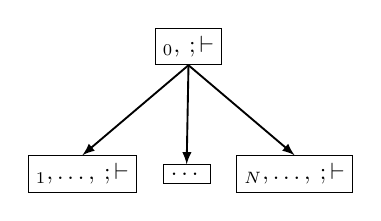
\begin{tikzpicture}[
  level distance=.75in,
  sibling distance=.15in,
  % auto,
  scale=0.85,
  edge from parent/.style={draw, thick,-latex},
  every tree node/.style={draw, align=center},
  grow'=down
]
\Tree
[.{$\sconstr_0,\:\cEnv ; \icEnv \solverRule \sconstr$}
  \edge node    { };
  [.{$\sconstr_N,\dots,\:\cEnv ; \icEnv \solverRule \sconstr$}
  ]
  \edge node[] { };
  [.{\dots}
  ]
  \edge node    { };
  [.{$\sconstr_1,\dots,\:\cEnv ; \icEnv \solverRule \sconstr$}
  ]
]
\end{tikzpicture}
$\qquad$
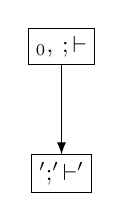
\begin{tikzpicture}[
  level distance=.75in,
  sibling distance=.15in,
  % auto,
  scale=0.85,
  edge from parent/.style={draw, thick,-latex},
  every tree node/.style={draw, align=center},
  grow'=down
]
\Tree
[.{$\sconstr_0,\:\cEnv ; \icEnv \solverRule \sconstr$}
  \edge node    { };
  [.{$\cEnv' ; \icEnv' \solverRule \sconstr'$}
  ]
]
\end{tikzpicture}
\\ \\ \\
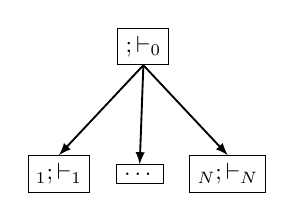
\begin{tikzpicture}[
  level distance=.75in,
  sibling distance=.15in,
  % auto,
  scale=0.85,
  edge from parent/.style={draw, thick,-latex},
  every tree node/.style={draw, align=center},
  grow'=down
]
\Tree
[.{$\emptyenv ; \icEnv \solverRule \sconstr_0$}
  \edge node    { };
  [.{$\cEnv_N; \icEnv \solverRule \sconstr_N$}
  ]
  \edge node[] { };
  [.{\dots}
  ]
  \edge node    { };
  [.{$\cEnv_1 ; \icEnv \solverRule \sconstr_1$}
  ]
]
\end{tikzpicture}
$\qquad$
      \fromany{$
      \inference{
        \sconstr \text{ jest trywialne}
      }{
        \emptyenv ; \icEnv \solverRule \sconstr
      }
      $}
$\qquad$
      \fromany{$
      \inference{
      \sconstr \in \icEnv
      }{
        \emptyenv ; \icEnv \solverRule \sconstr
      }$}
    \end{tabularx}
\end{frame}

\begin{frame}
\begin{tabularx}{\textwidth}{c|C}
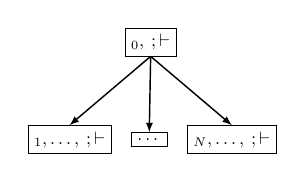
\begin{tikzpicture}[
  level distance=.75in,
  sibling distance=.15in,
  % auto,
  scale=0.65,
  edge from parent/.style={draw, thick,-latex},
  every tree node/.style={draw, align=center},
  grow'=down
]
\Tree
[.{$\sconstr_0,\:\cEnv ; \icEnv \solverRule \sconstr$}
  \edge node    { };
  [.{$\sconstr_N,\dots,\:\cEnv ; \icEnv \solverRule \sconstr$}
  ]
  \edge node[] { };
  [.{\dots}
  ]
  \edge node    { };
  [.{$\sconstr_1,\dots,\:\cEnv ; \icEnv \solverRule \sconstr$}
  ]
]
\end{tikzpicture}
& $
    \inference{
      \atomv \cneq \atomexp_1, \atomv \cneq \atomexp_2, \atomv     \ceq \atomexp, \cEnv ; \icEnv \vDash \sconstr \\
      \atomv \ceq  \atomexp_1, \atomv \cneq \atomexp_2, \atomexp_2 \ceq \atomexp, \cEnv ; \icEnv \vDash \sconstr \\
                              \atomv \ceq  \atomexp_2, \atomexp_1 \ceq \atomexp, \cEnv ; \icEnv \vDash \sconstr
    }{
      \atomv \ceq \permswap{\atomexp_1}{\atomexp_2} \atomexp, \cEnv ; \icEnv \vDash \sconstr
    }
  $
\\ &  \\ \hline & \\
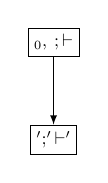
\begin{tikzpicture}[
  level distance=.75in,
  sibling distance=.15in,
  % auto,
  scale=0.65,
  edge from parent/.style={draw, thick,-latex},
  every tree node/.style={draw, align=center},
  grow'=down
]
\Tree
[.{$\sconstr_0,\:\cEnv ; \icEnv \solverRule \sconstr$}
  \edge node    { };
  [.{$\cEnv' ; \icEnv' \solverRule \sconstr'$}
  ]
]
\end{tikzpicture}
& \begin{tabular}{c}
  $
    \inference{
      \cEnv\subst{\termv}{\term} ; \icEnv\subst{\termv}{\term}
        \solverRule \sconstr\subst{\termv}{\term} \\ { }
    }{
      \termv = \term, \cEnv ; \icEnv \solverRule \sconstr
    % }\:\scbrk{Subst}{Term}$ \\ \\
    }
  $
  \end{tabular}
\\ & \\ \hline & \\ & \\ \dots & \dots \\ & \\
    \end{tabularx}
\end{frame}

% \begin{frame}
% The curious reader should now feel obliged to ask themselves a very important
% question: does the Solver's procedure always stop?
% To address this question, we define the state of the Solver as a triple ($\cEnv$, $\icEnv$, C).
% Upon analyzing the Solver rules, it becomes evident that each rule consistently leads
% to a lesser state by reducing it through one or more of the following actions:
% 1. Decreasing the number of distinct variables in $\cEnv$, $\icEnv$, and C, or maintaining the
% same number while:
% 2. Decreasing the depth of C, or preserving the current depth while:
% 3. Reducing assumptions with a given depth in either $\cEnv$ or $\icEnv$ into assumptions
% with lower depth, or maintaining the number and depth of assumptions, while:
% 4. Eliminating an assumption from $\cEnv$ and introducing an assumption of the same
% depth into $\icEnv$.
% That concludes the definition of the Solver. In the following chapters, when
% we write $\cEnv$ $\vDash$ c, we actually mean $\cEnv$; $\emptyenv$ $\solverRule$ C. This equivalence is established by the
% construction of $\solverRule$, which aligns with the interpretation of $\vDash$ as defined in the model.
% \end{frame}

\begin{frame}
\frametitle{Logika wyższego rzędu}
\large
\begin{tabularx}{\textwidth}{rL}
$\varphi \:\deff$
  & $\top \bnfor \bot
          \bnfor \formphi \vee \formphi
          \bnfor \formphi \wedge \formphi
          \bnfor \formphi \fImp \formphi$ \\
       \onslide<2->{
       & $\bnfor \fForallAtom{\atomv} \formphi
          \bnfor \fForallTerm{\termv} \formphi
          \bnfor \fForallProp{\propv}{\kind} \formphi$ \\
       & $\bnfor \fExistsAtom{\atomv} \formphi
          \bnfor \fExistsTerm{\termv} \formphi
          \bnfor \fExistsProp{\propv}{\kind} \formphi$ \\}
      \onslide<3->{
       & $ \bnfor \fLamAtom{\atomv} \formphi
          \bnfor \fLamTerm{\termv} \formphi
          \bnfor \fLamForm{\propv}{\kind} \formphi$ \\
       & $\bnfor \propv
          \bnfor \formphi \fAppAtom{\atomexp}
          \bnfor \formphi \fAppTerm{\term}
          \bnfor \formphi \fApp \formphi$ \\ }
       \onslide<4->{
       & $\bnfor \fConstr{\constr}
          \bnfor \fCAnd{\constr} \formphi
          \bnfor \fCImp{\constr} \formphi$ \\ }
       \onslide<5->{
       & $\bnfor \fix{\propv}{\termv}{\kind}{\formphi} $ \\ }
\end{tabularx}
\end{frame}

\begin{frame}
\frametitle{Dedukcja naturalna}
  \begin{tabularx}{\textwidth}{C|C}
  $
  \inference{
    \formphi \in \Theta
  }{
    \jgmnt[\cEnv;\Theta]{\formphi}
  }\scbrk{}{Assumption}
  $ & $
  \inference{
    \cjgmnt[\cEnv]{\constr}
  }{
    \jgmnt[\cEnv;\Theta]{\constr}
  }\scbrk{}{ConstrI}
  $ \\ & \\ & \\  $
  \inference{
    \jgmnt[\cEnv;\Theta,\formphi_1]{\formphi_2}
  }{
    \jgmnt[\cEnv;\Theta]{\formphi_1 \fImp \formphi_2}
  }\scbrk{}{ImpI}
  $ & $
  \inference{
    \jgmnt[\cEnv, \constr;\Theta]{\formphi}
  }{
    \jgmnt[\cEnv;\Theta]{\fCImp{\constr}\formphi}
  }\scbrk{Constr}{ImpI}
  $ \\ & \\ & \\ $
  \inference{
    \jgmnt[\cEnv_1;\Theta_1]{\formphi_1} &
    \jgmnt[\cEnv_2;\Theta_2]{\formphi_2}
  }{
    \jgmnt[\cEnv_1 \cup \cEnv_2;\Theta_2 \cup \Theta_2]{\formphi_1 \wedge \formphi_2}
  }\scbrk{}{AndI}
  $ & $
  \inference{
    \jgmnt[\cEnv_1;\Theta_1]{\constr} &
    \jgmnt[\cEnv_2;\Theta_2]{\formphi}
  }{
    \jgmnt[\cEnv_1 \cup \cEnv_2;\Theta_2 \cup \Theta_2]{\fCAnd{\constr}\formphi}
  }\scbrk{Constr}{AndI}
  $
  \end{tabularx}
\end{frame}

\begin{frame}
\frametitle{Aksjomaty}
  \begin{tabularx}{\textwidth}{C}
  $
  \inference{
  }{
    \jgmnt[]{\fForallAtom{\:\atomv,\:\atomv'} (\atomv \ceq \atomv') \vee (\atomv \cneq \atomv')}
  }\:\scbrk{Axiom}{Compare}
  $ \\ \\ \\ $
  \inference{
  }{
    \jgmnt[]{\fForallTerm{\termv} \:\fExistsAtom{\atomv} (\atomv \cfresh \termv)}
  }\:\scbrk{Axiom}{Fresh}
  $ \\ \\ \\ $
  \inference{
  }{
    \jgmnt[]{\fForallTerm{\termv} (\fExistsAtom{\atomv}\: \termv = \atomv) \vee (\fExistsAtom{\atomv}\:\fExistsTerm{\termv'}\: \termv = \tbind{\atomv}{\termv'}) }
  }\:\scbrk{Axiom}{Inversion} $ \\
  $\vee \: (\fExistsTerm{\termv_1,\:\termv_2}\: \termv = \termv_1 \tapp \termv_2) \vee ({symbol}\: \termv) \qquad\qquad
  $ \\ \\ \\ $
  \inference{
    \jgmnt[\cEnv;\Theta, (\fForallTerm{\termv'} \fCImp{\termv' \cshlt \termv} \formphi(\termv'))]{\formphi(\termv)}
    }{
    \jgmnt[\cEnv;\Theta]{\fForallTerm{\termv} \formphi(\termv)}
  }\:\scbrk{Induction}{}
  $
  \end{tabularx}
\end{frame}

\begin{frame}
\frametitle{Indukcja}
  \begin{tabularx}{\textwidth}{L}
  $ \hfill
  \term \; \deff \; \atomexp
                         \mid \perm \apperm \termv
                         \mid \tbind{\atomexp} \term
                         \mid \term \tapp \term
                         \mid \symb
      \quad \text{(termy)}
  $ \\ \\ $
  \inference{
    \jgmnt[\cEnv;\Theta, (\fForallTerm{\termv'} \fCImp{\termv' \cshlt \termv} \formphi(\termv'))]{\formphi(\termv)}
    }{
    \jgmnt[\cEnv;\Theta]{\fForallTerm{\termv} \formphi(\termv)}
  }\:\scbrk{}{Induction}
  $ \\ \\ $
  \
  $ \\
  \only<2-3>{
  \begin{tabular}{l}
  $\fForallProp{P \ofkind (\kForallTerm{\termv}{\kProp})\:}{}$ \\
  $\phantom{\fImp}\;(\fForallAtom{\atomv} P({\atomv}))$ \\
  $\fImp          (\fForallTerm{\termv_1, \termv_2} P ({\termv_1}) \fImp P ({\termv_2}) \fImp P({\termv_1 \tapp \termv_2}))$ \\
  $\fImp$
  \hspace{-1.25mm}\only<2>{
    $(\fForallAtom{\atomv}\fForallTerm{\termv} P ({\termv}) \fImp P({\tbind{\atomv}{\termv}}))$
  }
  \hspace{-1.25mm}\only<3>{
    $(${\color{red}$\fForallTerm{C}$}$\fForallAtom{\atomv}\fForallTerm{\termv}${\color{red}$\fCImp{\atomv \cfresh {C} }$}$\:P ({\termv}) \fImp P({\tbind{\atomv}{\termv}}))$
  } \\
  $\fImp          (\fForallTerm{\termv} \fCImp{\csymb \termv}{P ({\termv})})$ \\
  $\quad \fImp \fForallTerm{\termv} {P ({\termv})}$ \\
  \end{tabular}
  }
  \end{tabularx}
\end{frame}

\begin{frame}
\frametitle{Rekursja --- punkt stały}
\begin{tabularx}{\textwidth}{C}
$
(\fix{\propv}{\termv}{\kind}{\formphi})\fApp\term
\;\equiv\;
\formphi\subst{\termv}{\term}\subst{\propv}{(\fix{\propv}{\termv}{\kind}{\formphi})}
\quad\:\scbrk{Fixpoint}{Unwrap}
$ \\ \\
  \onslide<2->{
$
\inference{
  \cEnv;\kEnv, (\propv \ofkind \kForallTerm{Y} \kGuard{Y \cshlt \termv}{\kind\subst{\termv}{Y}})\vdash \formphi \ofkind \kind
}{
  \cEnv;\kEnv\vdash (\fix{\propv}{\termv}{\kind}{\formphi}) \ofkind \kForallTerm{\termv}{\kind}
}\:\scbrk{Kind}{Fixpoint}
$ \\ \\ \\ $}
  \onslide<3->{
\inference{
  }{
    \cEnv; \kEnv \vdash \fConstr{\constr} \ofkind \kProp
    }\:\scbrk{Kind}{Constr}
  \qquad
  \inference{
    \cEnv,\constr; \kEnv \vdash \formphi \ofkind \kProp
  }{
    \cEnv; \kEnv \vdash \fCAnd{\constr} \formphi \ofkind \kProp
    }\:\scbrk{Kind}{ConstrAnd}
  $ \\ \\ \\ $
    \inference{
      \cEnv;\kEnv\vdash \formphi \ofkind \kForallTerm{\termv}\kind
    }{
      \cEnv;\kEnv\vdash \formphi \fAppTerm{\term} \ofkind \kind\subst{\termv}{\term}
    }\:\scbrk{Kind}{AppTerm}
    \qquad
    \inference{
          \cEnv \vDash \constr
        }{
          \cEnv \vdash \kGuard{\constr}\kind \subkind \kind
        }\:\scbrk{Subkind}{Reduce}
  $}
\end{tabularx}
\end{frame}

\begin{frame}
\frametitle{Implementacja}
  \begin{tabularx}{\linewidth}{|c|X|}
    \hline & \\
    \tt{Proof}
      & ``Interfejs dla sprawdzającego dowód'':
          dedukcja naturalna zaimplementowana w postaci smart-konstruktorów
          abstrakcyjnego typu danych \tt{proof}. \\ & \\
    \hline & \\
    \tt{IncProof}
      & ``Interfejs dla prowadzącego dowód'':
          drzewa niepełnych dowodów. \\ & \\
    \hline & \\
    \tt{Prover}
      & ``Interfejs dla człowieka'':
          asystent dowodzenia. \\ & \\
    \hline
  \end{tabularx}
\end{frame}

\lstset{literate={ż}{{\.z}}1}

% \begin{frame}[fragile]
% \frametitle{Studium przypadku: rachunek lambda z typami prostymi}
%   \begin{tabular}{l}
%   $\fForallProp{P \ofkind (\kForallTerm{\termv}{\kProp})\:}{}$ \\
%   $\phantom{\fImp}\;(\fForallAtom{\atomv} P({\atomv}))$ \\
%   $\fImp          (\fForallTerm{\termv_1, \termv_2} P ({\termv_1}) \fImp P ({\termv_2}) \fImp P({\termv_1 \tapp \termv_2}))$ \\
%   $\fImp          (\fForallTerm{C} \fForallAtom{\atomv}\fForallTerm{\termv} \fCImp{\atomv \cfresh {C}}\:P ({\termv}) \fImp P({\tbind{\atomv}{\termv}}))$
%   \\
%   $\fImp          (\fForallTerm{\termv} \fCImp{\csymb \termv}{P ({\termv})})$ \\
%   $\quad \fImp \fForallTerm{\termv} {P ({\termv})}$
% \end{tabular}
% \\ test \\
% \begin{tabular}{ll}
%   \hspace{2cm}
%   \begin{tabular}{l}
%   $\fForallProp{P \ofkind (\kForallTerm{\termv}{\kProp})\:}{}$ \\
%   $\phantom{\fImp}\;(\fForallAtom{\atomv} P({\atomv}))$ \\
%   $\fImp          (\fForallTerm{\termv_1, \termv_2} P ({\termv_1}) \fImp P ({\termv_2}) \fImp P({\termv_1 \tapp \termv_2}))$ \\
%   $\fImp          (\fForallTerm{C} \fForallAtom{\atomv}\fForallTerm{\termv} \fCImp{\atomv \cfresh {C}}\:P ({\termv}) \fImp P({\tbind{\atomv}{\termv}}))$
%   \\
%   $\fImp          (\fForallTerm{\termv} \fCImp{\csymb \termv}{P ({\termv})})$ \\
%   $\quad \fImp \fForallTerm{\termv} {P ({\termv})}$ \\
%   \end{tabular}
%   \end{tabular}
% \end{frame}

\begin{frame}[fragile]
\frametitle{Studium przypadku: rachunek lambda z typami prostymi}
\begin{lstlisting}[mathescape,language=OCaml,escapebegin=\color{codepurple}]

let lambda_symbols = (* symbole używane w formalizacji STLC *)
  ["lam"; "app"; "base"; "arrow"; "nil"; "cons"]

let term_predicate = (* Term e *)
  "fix Term(e): * =
   var: ($\exists$ a :atom. (e = a))
   $\vee$
   lam: ($\exists$ a :atom. $\exists$ e' :term. [e = lam (a.e')] $\wedge$ (Term e'))
   $\vee$
   app: ($\exists$ e1 e2 :term. [e = app e1 e2] $\wedge$ (Term e1) $\wedge$ (Term e2))"

let type_predicate = (* Type t *)
  "fix Type(t): * =
   base: (t = base)
   $\vee$
   arrow: ($\exists$ t1 t2 :term. [t $\ceq$ arrow t1 t2]
             $\wedge$ (Type t1) $\wedge$ (Type t2))"
\end{lstlisting}
\end{frame}

% Czy ctx może być na początku twierdzenia? A chuj niech będzie
\begin{frame}[fragile]
\frametitle{Indukcja dla $\lambda$-termów}
\begin{lstlisting}[mathescape,language=OCaml,escapebegin=\color{codepurple}]
let term_predicate = (* Term e *)
  "fix Term(e): * =
   var: ($\exists$ a :atom. (e = a))
   $\vee$
   lam: ($\exists$ a :atom. $\exists$ e' :term. [e = lam (a.e')] $\wedge$ (Term e'))
   $\vee$
   app: ($\exists$ e1 e2 :term. [e = app e1 e2] $\wedge$ (Term e1) $\wedge$ (Term e2))"

let lambda_ind_thm = lambda_thm
  "$\forall$ P : ($\forall$ _ :term. prop).
   $\forall$ ctx : term.
        ($\forall$ a :atom. P {a})
     $\fImp$ ($\forall$ e1 e2 :term. (Term e1) $\fImp$ (Term e2) $\fImp$
          (P e1) $\fImp$ (P e2) $\fImp$ P {app t1 t2})
     $\fImp$ ($\forall$ a :atom. $\forall$ e :term. (Term e) $\fImp$
          [a # ctx] $\fImp$ (P e) $\fImp$ P {lam (a.e)})
     $\fImp$ $\forall$ e :term. (Term e) $\fImp$ P e
\end{lstlisting}
\end{frame}

% \begin{frame}[fragile]
% \begin{lstlisting}[mathescape,language=OCaml,escapebegin=\color{codepurple}]
% let typing_relation = (* Typing e env t *)
%   "fix Typing(e): $\forall$ env t :term. * =
%    fun env t :term $\rightarrow$
%      var: ($\exists$ a :atom. [e = a] $\wedge$ (InEnv env a t))
%      $\vee$
%      lam: ($\exists$ a :atom.$\exists$ e' t1 t2 :term.
%             [e = lam (a.e')] $\wedge$ [t = arrow t1 t2]
%               $\wedge$ (Type t1) $\wedge$ (Typing e' {cons a t1 env} t2))
%      $\vee$
%      app: ($\exists$ e1 e2 t2 :term. [e = app e1 e2]
%             $\wedge$ (Typing e1 env {arrow t2 t}) $\wedge$ (Typing e2 env t2))"

% let inenv_relation = (* InEnv env a t *)
%   "fix InEnv(env): $\forall$ a :atom. $\forall$ t :term. * =
%    fun (a :atom) (t :term) $\rightarrow$
%      current: ($\exists$ env': term. env = cons a t env')
%      $\vee$
%      next: ($\exists$ b :atom. $\exists$ s env': term.
%             [env = cons b s env'] $\wedge$ [a $\cneq$ b] $\wedge$ (InEnv env' a t))"
% \end{lstlisting}
% \end{frame}

% \begin{frame}[fragile]
% \begin{lstlisting}[mathescape,language=OCaml,escapebegin=\color{codepurple}]
% let empty_contradiction_thm = lambda_thm
%   "forall a :atom.
%    forall t :term.
%      (InEnv nil a t) $\fImp$ false"
% \end{lstlisting}

% \begin{overlayarea}{\linewidth}{3cm}
% \begin{onlyenv}<1>
% \begin{lstlisting}[mathescape,language=OCaml,escapebegin=\color{codepurple}]
%   let empty_contradiction =
%   proof' empty_contradiction_thm
% \end{lstlisting}
% \end{onlyenv}
%   \begin{onlyenv}<2>
%   \begin{lstlisting}[mathescape,language=OCaml,escapebegin=\color{codepurple}]
%   let empty_contradiction =
%   proof' empty_contradiction_thm
%   |> intros ["a"; "t"; "H"]
% \end{lstlisting}
% \end{onlyenv}
%   \begin{onlyenv}<3>
%   \begin{lstlisting}[mathescape,language=OCaml,escapebegin=\color{codepurple}]
%   let empty_contradiction =
%   proof' empty_contradiction_thm
%   |> intros ["a"; "t"; "H"] %> destruct_assm "H"
% \end{lstlisting}
% \end{onlyenv}
%   \begin{onlyenv}<4>
%   \begin{lstlisting}[mathescape,language=OCaml,escapebegin=\color{codepurple}]
%   let empty_contradiction =
%   proof' empty_contradiction_thm
%   |> intros ["a"; "t"; "H"] %> destruct_assm "H"
%   |> intros' ["contra"; "env'"]
% \end{lstlisting}
% \end{onlyenv}
%   \begin{onlyenv}<5>
%   \begin{lstlisting}[mathescape,language=OCaml,escapebegin=\color{codepurple}]
%   let empty_contradiction =
%   proof' empty_contradiction_thm
%   |> intros ["a"; "t"; "H"] %> destruct_assm "H"
%   |> intros' ["contra"; "env'"] %> discriminate
% \end{lstlisting}
% \end{onlyenv}
%   \begin{onlyenv}<6>
%   \begin{lstlisting}[mathescape,language=OCaml,escapebegin=\color{codepurple}]
%   let empty_contradiction =
%   proof' empty_contradiction_thm
%   |> intros ["a"; "t"; "H"] %> destruct_assm "H"
%   |> intros' ["contra"; "env'"] %> discriminate
%   |> intros' ["contra"; "b"; "s"; "env'"; ""]
% \end{lstlisting}
% \end{onlyenv}
%   \begin{onlyenv}<7>
%   \begin{lstlisting}[mathescape,language=OCaml,escapebegin=\color{codepurple}]
%   let empty_contradiction =
%   proof' empty_contradiction_thm
%   |> intros ["a"; "t"; "H"] %> destruct_assm "H"
%   |> intros' ["contra"; "env'"] %> discriminate
%   |> intros' ["contra"; "b"; "s"; "env'"; ""] %> solve
% \end{lstlisting}
% \end{onlyenv}
%   \begin{onlyenv}<8>
%   \begin{lstlisting}[mathescape,language=OCaml,escapebegin=\color{codepurple}]
%   let empty_contradiction =
%   proof' empty_contradiction_thm
%   |> intros ["a"; "t"; "H"] %> destruct_assm "H"
%   |> intros' ["contra"; "env'"] %> discriminate
%   |> intros' ["contra"; "b"; "s"; "env'"; ""] %> solve
%   |> qed
% \end{lstlisting}
% \end{onlyenv}
% \end{overlayarea}
% \begin{overlayarea}{\linewidth}{2cm}
%   \begin{onlyenv}<1>
%   \begin{lstlisting}[mathescape]
% Unfinished:

% [ ]
% [ ]
% $\vdash$ $\forall$ a : atom. $\forall$ t : term. (InEnv nil a t) $\fImp$ $\bot$
% \end{lstlisting}
% \end{onlyenv}
%   \begin{onlyenv}<2>
%   \begin{lstlisting}[mathescape]
% Unfinished:

% [ ]
% [ H : InEnv nil a t ]
% $\vdash$ $\bot$
% \end{lstlisting}
% \end{onlyenv}
%   \begin{onlyenv}<3>
%   \begin{lstlisting}[mathescape]
% Unfinished:

% [ ]
% [ ]
% $\vdash$ ($\exists$ env' : term. (nil = cons a t env')) $\fImp$ $\bot$
% \end{lstlisting}
% \end{onlyenv}
%   \begin{onlyenv}<4>
%   \begin{lstlisting}[mathescape]
% Unfinished:

% [ ]
% [ contra : (nil = cons a t env') ]
% $\vdash$ $\bot$
% \end{lstlisting}
% \end{onlyenv}
%   \begin{onlyenv}<5>
%   \begin{lstlisting}[mathescape]
% Unfinished:

% [ ]
% [ ]
% $\vdash$ ($\exists$ b : atom. $\exists$ s env' : term.
%      [nil = cons b s env'] $\wedge$ [a =/= b] $\wedge$ InEnv env' a t)
%       $\fImp$ $\bot$
% \end{lstlisting}
% \end{onlyenv}
%   \begin{onlyenv}<6>
%   \begin{lstlisting}[mathescape]
% Unfinished:

% [ nil = cons b s env' ]
% [ contra : [a =/= b] $\wedge$ InEnv env' a t ]
% $\vdash$ $\bot$
% \end{lstlisting}
% \end{onlyenv}
%   \begin{onlyenv}<7>
%   \begin{lstlisting}[mathescape]
% Finished:

% [ ]
% [ ]
% $\vdash$ $\forall$ a : atom. $\forall$ t : term. (InEnv nil a t) $\fImp$ $\bot$
% \end{lstlisting}
% \end{onlyenv}
% \end{overlayarea}
% \end{frame}

% \begin{frame}[fragile]
% \begin{lstlisting}[mathescape,language=OCaml,escapebegin=\color{codepurple}]
% let value_predicate = (* Value v *)
%   "fun e :term $\rightarrow$
%      var: ($\exists$ a :atom. [e = a])
%      $\vee$
%      lam: ($\exists$ a :atom. $\exists$ e' : term. [e = lam (a.e')] $\wedge$ (Term e'))"

% let steps_relation = (* Steps e e' *)
%   "fix Steps(e): $\forall$ e' :term.* = fun e' :term $\rightarrow$
%      app_l: ($\exists$ e1 e1' e2 :term. [e = app e1 e2]
%               $\wedge$ [e' = app e1' e2] $\wedge$ (Steps e1 e1') )
%      $\vee$
%      app_r: ($\exists$ v e2 e2' :term. [e = app v e2]
%               $\wedge$ [e' = app v e2'] $\wedge$ (Value v) $\wedge$ (Steps e2 e2') )
%      $\vee$
%      app: ($\exists$ a :atom.$\exists$ e_a v :term. [e = app (lam (a.e_a)) v]
%             $\wedge$ (Value v) $\wedge$ (Sub e_a a v e') )"

% let progressive_predicate = (* Progressive e *)
%   "fun e:term $\rightarrow$
%      value: (Value e) $\vee$ steps: ($\exists$ e' :term. Steps e e')"
% \end{lstlisting}
% \end{frame}


% \begin{frame}[fragile]
% \begin{lstlisting}[mathescape,language=OCaml,escapebegin=\color{codepurple}]
% let progress_thm = lambda_thm
%   "$\forall$ e t :term. (Typing e nil t) $\fImp$ (Progressive e)"


% let canonical_form_thm = lambda_thm
%   "$\forall$ v :term. (Value v) $\fImp$
%    $\forall$ t :term. (Typing v nil t) $\fImp$
%      ($\exists$ a :atom. $\exists$ e :term. [v = lam (a.e)] $\wedge$ (Term e))"
% \end{lstlisting}
% \end{frame}

% \begin{frame}[fragile]
% \begin{overlayarea}{\linewidth}{3.5cm}
%   \begin{onlyenv}<1>
%   \begin{lstlisting}[mathescape,language=OCaml,escapebegin=\color{codepurple}]
% let canonical_form =
%   proof' canonical_form_thm
%   |> intros ["v"; "t"; "Hv"]
% \end{lstlisting}
% \end{onlyenv}
% \begin{onlyenv}<2>
%   \begin{lstlisting}[mathescape,language=OCaml,escapebegin=\color{codepurple}]
% let canonical_form =
%   proof' canonical_form_thm
%   |> intros ["v"; "t"; "Hv"] %> intro'
% \end{lstlisting}
% \end{onlyenv}
%   \begin{onlyenv}<3>
%   \begin{lstlisting}[mathescape,language=OCaml,escapebegin=\color{codepurple}]
% let canonical_form =
%   proof' canonical_form_thm
%   |> intros ["v"; "t"; "Hv"] %> intro'
%   |> intros' ["contra"; "a"; ""]
% \end{lstlisting}
% \end{onlyenv}
%   \begin{onlyenv}<4>
%   \begin{lstlisting}[mathescape,language=OCaml,escapebegin=\color{codepurple}]
% let canonical_form =
%   proof' canonical_form_thm
%   |> intros ["v"; "t"; "Hv"] %> intro'
%   |> intros' ["contra"; "a"; ""]
%      %> ex_falso
%      %> apply_thm_spec empty_contradiction ["a"; "t"]
%      %> assumption
% \end{lstlisting}
% \end{onlyenv}
%   \begin{onlyenv}<5>
%   \begin{lstlisting}[mathescape,language=OCaml,escapebegin=\color{codepurple}]
% let canonical_form =
%   proof' canonical_form_thm
%   |> intros ["v"; "t"; "Hv"] %> intro'
%   |> intros' ["contra"; "a"; ""] ...
%   |> intros' ["Hlam"; "a"; "e"; "t1"; "t2"; ""; ""; ""]
% \end{lstlisting}
% \end{onlyenv}
%   \begin{onlyenv}<6>
%   \begin{lstlisting}[mathescape,language=OCaml,escapebegin=\color{codepurple}]
% let canonical_form =
%   proof' canonical_form_thm
%   |> intros ["v"; "t"; "Hv"] %> intro'
%   |> intros' ["contra"; "a"; ""] ...
%   |> intros' ["Hlam"; "a"; "e"; "t1"; "t2"; ""; ""; ""]
%      %> exists' ["a"; "e"] %> solve
% \end{lstlisting}
% \end{onlyenv}
%   \begin{onlyenv}<7>
%   \begin{lstlisting}[mathescape,language=OCaml,escapebegin=\color{codepurple}]
% let canonical_form =
%   proof' canonical_form_thm
%   |> intros ["v"; "t"; "Hv"] %> intro'
%   |> intros' ["contra"; "a"; ""] ...
%   |> intros' ["Hlam"; "a"; "e"; "t1"; "t2"; ""; ""; ""]
%      %> exists' ["a"; "e"] %> solve
%      %> apply_thm_spec typing_terms ["e"; "cons a t1 nil"; "t2"]
%      %> assumption
% \end{lstlisting}
% \end{onlyenv}
%   \begin{onlyenv}<8>
%   \begin{lstlisting}[mathescape,language=OCaml,escapebegin=\color{codepurple}]
% let canonical_form =
%   proof' canonical_form_thm
%   |> intros ["v"; "t"; "Hv"] %> intro'
%   |> intros' ["contra"; "a"; ""]
%      %> ex_falso
%      %> apply_thm_spec empty_contradiction ["a"; "t"]
%      %> assumption
%   |> intros' ["Hlam"; "a"; "e"; "t1"; "t2"; ""; ""; ""]
%      %> exists' ["a"; "e"] %> solve
%      %> apply_thm_spec typing_terms ["e"; "cons a t1 nil"; "t2"]
%      %> assumption
%   |> intros' ["contra"; "e1"; "e2"; "t2"; ""]
%      %> ex_falso
%      %> destruct_assm "Hv"
%      %> (intros' ["contra_var"; "a"] %> discriminate)
%      %> (intros' ["contra_lam"; "a"; "e"; ""] %> discriminate)
%   |> qed
% \end{lstlisting}
% \end{onlyenv}
% \end{overlayarea}
% \begin{overlayarea}{\linewidth}{2cm}
%   \begin{onlyenv}<1>
%   \begin{lstlisting}[mathescape]
% Unfinished:

% [ ]
% [ Hv : Value v ]
% $\vdash$ (Typing v nil t) $\fImp$
%     $\exists$ a : atom. $\exists$ e : term. [v = lam (a.e)] $\wedge$ Term e
% \end{lstlisting}
% \end{onlyenv}
%   \begin{onlyenv}<2>
%   \begin{lstlisting}[mathescape]
% Unfinished:

% [ ]
% [ Hv : Value v ]
% $\vdash$ ($\exists$ a : atom. [v = a] $\wedge$ InEnv nil a t)
%     $\exists$ a : atom. $\exists$ e : term. [v = lam (a.e)] $\wedge$ Term e
% \end{lstlisting}
% \end{onlyenv}
%   \begin{onlyenv}<3>
%   \begin{lstlisting}[mathescape]
% Unfinished:

% [ v = a ]
% [ Hv : Value v ; contra : InEnv nil a t ]
% $\vdash$ $\exists$ a'1 : atom. $\exists$ e : term. [v = lam (a'1.e)] $\wedge$ Term e
% \end{lstlisting}
% \end{onlyenv}
%   \begin{onlyenv}<4>
%   \begin{lstlisting}[mathescape]
% Unfinished:

% [ ]
% [ Hv : Value v ]
% $\vdash$ ($\exists$ a : atom. $\exists$ e' t1 t2 : term.
%     [v = lam (a.e')] $\wedge$ [t = arrow t1 t2]
%     $\wedge$ Type t1 $\wedge$ Typing e' {cons a t1 nil} t2)
%       $\fImp$ $\exists$ a : atom. $\exists$ e : term. [v = lam (a.e)] $\wedge$ Term e
% \end{lstlisting}
% \end{onlyenv}
%   \begin{onlyenv}<5>
%   \begin{lstlisting}[mathescape]
% Unfinished:

% [ v = lam (a.e) ; t = arrow t1 t2 ]
% [
%   Hlam_2 : Typing e {cons a t1 nil} t2 ;
%   Hlam_1 : Type t1 ;
%   Hv : Value v
% ]
% $\vdash$ $\exists$ a'1 : atom. $\exists$ e'1 : term. [v = lam (a'1.e'1)] $\wedge$ Term e'1
% \end{lstlisting}
% \end{onlyenv}
%   \begin{onlyenv}<6>
%   \begin{lstlisting}[mathescape]
% Unfinished:

% [ v = lam (a.e) ; t = arrow t1 t2 ]
% [
%   Hlam_2 : Typing e {cons a t1 nil} t2 ;
%   Hlam_1 : Type t1 ;
%   Hv : Value v
% ]
% $\vdash$ Term e
% \end{lstlisting}
% \end{onlyenv}
%   \begin{onlyenv}<7>
%   \begin{lstlisting}[mathescape]
% Unfinished:

% [ ]
% [ Hv : Value v ]
% $\vdash$ ($\exists$ e1 e2 t2 : term.
%     [v = app e1 e2] $\wedge$ Typing e1 nil {arrow t2 t}
%       $\wedge$ Typing e2 nil t2)
%       $\fImp$ $\exists$ a : atom. $\exists$ e : term. [v = lam (a.e)] $\wedge$ Term e
% \end{lstlisting}
% \end{onlyenv}
% \end{overlayarea}
% \end{frame}
% \begin{frame}[fragile]
% \begin{lstlisting}[mathescape,language=OCaml,escapebegin=\color{codepurple}]
% let preservation_thm = lambda_thm
%   "forall e e' env t :term.
%      (Typing e env t) $\fImp$
%      (Steps e e') $\fImp$
%        (Typing e' env t)"

% let sub_lemma_thm = lambda_thm
%   "$\forall$ e env t :term.
%    $\forall$ a : atom. $\forall$ ta :term.
%    $\forall$ v e' :term.
%      (Typing v env ta) $\fImp$
%      (Typing e {cons a ta env} t) $\fImp$
%      (Sub e a v e') $\fImp$
%        (Typing e' env t)"

% let weakening_lemma_thm = lambda_thm
%   "$\forall$ e env1 t env2 : term.
%      (Typing e env1 t) $\fImp$
%      (EnvInclusion env1 env2) $\fImp$
%        (Typing e env2 t)"
% \end{lstlisting}
% \end{frame}

\begin{frame}
\centering{
  \begin{tabularx}{\textwidth}{C}
    \it{\huge Live Demo}
    \\ \\
    ???
  \end{tabularx}
}
\end{frame}

\begin{frame}
\centering{
  \it{\huge Koniec}
}
\end{frame}


\end{document}
